\begin{frame}[t]
    \frametitle{Results: Canonical refining}
    \framesubtitle{Discovering \textit{de-novo} miRNAs}
    \begin{figure}[h!]
        \centering
        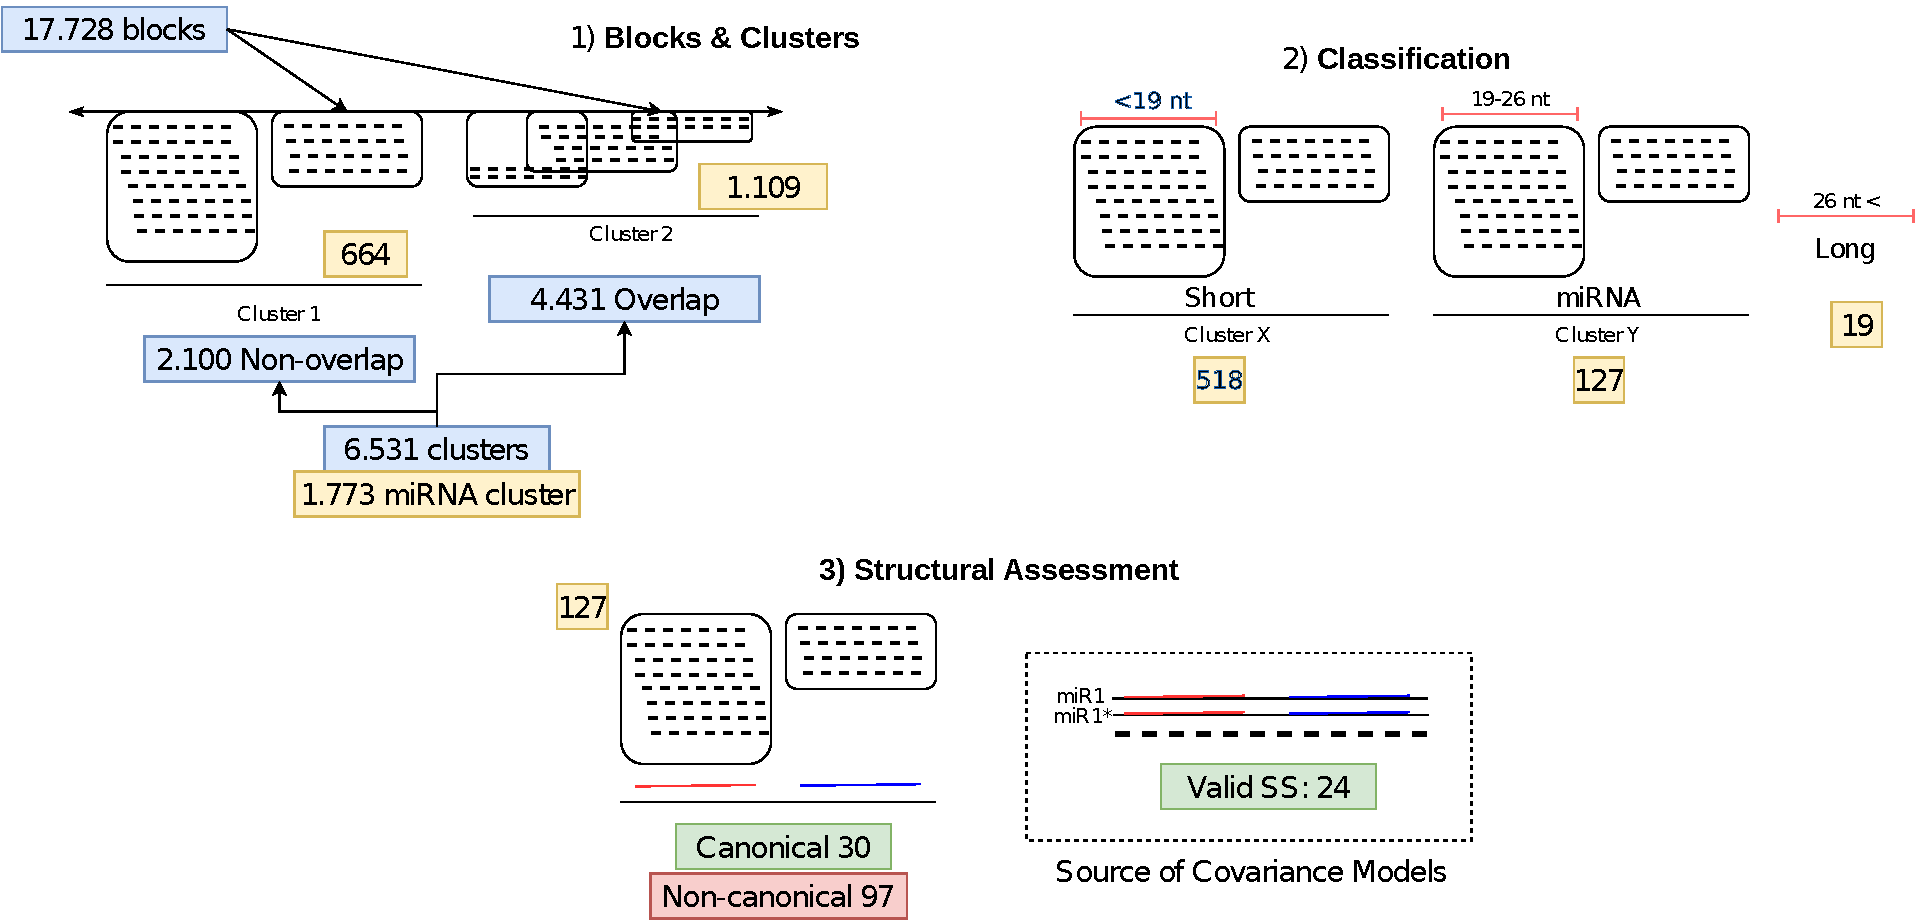
\includegraphics[width=\linewidth]{Figures/results_workflowALL}\label{fig:workflow} %
    \end{figure}
    \begin{itemize}
        \item Only $3.6$ \% potential candidates detected as \textit{canonical} miRNAs.
        \item Expression of potential piwi-RNAs covers most of the candidates ($\sim 77.4$\%)
    \end{itemize}
\end{frame}

\begin{frame}[t]
    % Take the most expressed candidates from the 24 ones and show one comparison.
    \frametitle{Disentangling miRNA annotation on \textit{C.\ robusta}}
    Example: Chromosome $7$ cluster ($30$ miRNA loci over $3713$ nt)
    \begin{figure}[h!]
        \centering
        \includegraphics<1>[width=\linewidth]{Figures/chr7_cluster} %
    \end{figure}
    \begin{itemize}
        \item $2$ covered by de-novo expression patterns.
        \item $X$ by homology annotation using \texttt{miRNAture}.
    \end{itemize}
\end{frame}

\begin{frame}[t]
    \frametitle{Results: Iteration $1$}
    \framesubtitle{Discovering \textit{de-novo} miRNAs}
    \begin{itemize}
        \item Starting point: $24$ CMs from \textit{C.\ robusta}.
        \item First target specie: \textit{Ciona savignyi}.
    \end{itemize}
\end{frame}

